\documentclass[a4paper]{article}
\usepackage[utf8x]{inputenc}
\usepackage[T1,T2A]{fontenc}
\usepackage[russian]{babel}
\usepackage{hyperref}
\usepackage{indentfirst}
\usepackage{listings}
\usepackage{color}
\usepackage{here}
\usepackage{array}
\usepackage{multirow}
\usepackage{graphicx}

\usepackage{caption}
\renewcommand{\lstlistingname}{Программа} % заголовок листингов кода

\usepackage{listings}
\lstset{ %
extendedchars=\true,
keepspaces=true,
language=bash,					% choose the language of the code
basicstyle=\footnotesize,		% the size of the fonts that are used for the code
numbers=left,					% where to put the line-numbers
numberstyle=\footnotesize,		% the size of the fonts that are used for the line-numbers
stepnumber=1,					% the step between two line-numbers. If it is 1 each line will be numbered
numbersep=5pt,					% how far the line-numbers are from the code
backgroundcolor=\color{white},	% choose the background color. You must add \usepackage{color}
showspaces=false				% show spaces adding particular underscores
showstringspaces=false,			% underline spaces within strings
showtabs=false,					% show tabs within strings adding particular underscores
frame=single,           		% adds a frame around the code
tabsize=2,						% sets default tabsize to 2 spaces
captionpos=b,					% sets the caption-position to bottom
breaklines=true,				% sets automatic line breaking
breakatwhitespace=false,		% sets if automatic breaks should only happen at whitespace
escapeinside={\%*}{*)},			% if you want to add a comment within your code
postbreak=\raisebox{0ex}[0ex][0ex]{\ensuremath{\color{red}\hookrightarrow\space}}
}

\usepackage[left=2cm,right=2cm,
top=2cm,bottom=2cm,bindingoffset=0cm]{geometry}

\begin{document}	% начало документа

\begin{titlepage}	% начало титульной страницы

	\begin{center}		% выравнивание по центру

		\large Санкт-Петербургский Политехнический Университет Петра Великого\\
		\large Институт компьютерных наук и технологий \\
		\large Кафедра компьютерных систем и программных технологий\\[6cm]
		% название института, затем отступ 6см
		
		\huge Программирование\\[0.5cm] % название работы, затем отступ 0,5см
		\large Отчет по курсовой работе \\[0.1cm]
		\large Игра "Мельница"\\[5cm]

	\end{center}


	\begin{flushright} % выравнивание по правому краю
		\begin{minipage}{0.25\textwidth} % врезка в половину ширины текста
			\begin{flushleft} % выровнять её содержимое по левому краю

				\large\textbf{Работу выполнила:}\\
				\large Власова А.В.\\
				\large {Группа:} 23501/4\\
				
				\large \textbf{Преподаватель:}\\
				\large Вылегжанина К.Д.

			\end{flushleft}
		\end{minipage}
	\end{flushright}
	
	\vfill % заполнить всё доступное ниже пространство

	\begin{center}
	\large Санкт-Петербург\\
	\large \the\year % вывести дату
	\end{center} % закончить выравнивание по центру

\thispagestyle{empty} % не нумеровать страницу
\end{titlepage} % конец титульной страницы

\vfill % заполнить всё доступное ниже пространство








% Содержание
\tableofcontents
\newpage



\section{Проектирование приложения для игры в Мельницу}

Мельница - логическая настольная игра для двух игроков, сохраняющая свою популярность уже более 3000 лет. Считается, что именно Мельница стала прародителем знаменитой игры "Крестики-нолики" из-за некоторого сходства в правилах. В наши дни Мельница остается известной среди любителей настольных игр. Традиционно для игры в Мельницу используют деревянную доску, однако в настоящее время для этой цели широко используются специальные приложения для компьютеров, смартфонов и других устройств.

\subsection{Задание}

Разработать Android-приложение, позволяющее двум игрокам играть в Мельницу.

\subsection{Концепция}

Готовое приложение дает возможность двум пользователям играть в Мельницу на Android-устройствах.

\subsection{Минимально работоспособный продукт}

Android-приложение, предназначенное для игры двух соперников в Мельницу.

\subsection{Правила}

Игра начинается с того, что оба игрока по очереди размещают по одной своей фишке на свободных кружках игрового поля. Каждый игрок имеет по 9 фишек. Если игроку удалось выставить три фишки в ряд на одной линии, он забирает любую фишку противника. Ряд из трех фишек называется мельницей.

После того, как все фишки будут размещены на поле, игроки начинают по очереди передвигать свои фишки на соседние кружки с целью построить мельницу. Перемещать фишки можно только по линиям, расположенным на поле. Когда у игрока остается только три фишки, он может перемещать их на любые свободные кружки не зависимо от линий. В это время его соперник продолжает ходить по старым правилам, пока у него тоже не останется три фишки.

Игра считается выигранной, когда соперник не может построить мельницу. Это может произойти, когда у противника осталось всего две фишки, или у него нет возможности сделать ход.

\subsection{Выделенные подпроекты}

В процессе проектирования приложения было выделено два подпроекта.

\begin{itemize}

\item \textbf{Core}

Библиотека, представляющая бизнес-логику приложения.

\item \textbf{app}

Android-приложение, обеспечивающее взаимодействие пользователей с ядром.

\end{itemize}

\subsection{Описание интерфейса библиотеки}

Интерфейс библиотеки содержит в себе следующие методы:

\begin{itemize}

\item Метод, позволяющий установить фишку на поле

\textbf{boolean makeMove(int x, int y, int z);}

\item Метод, позволяющий передвинуть фишку в доступную ячейку

\textbf{boolean makeMove( int fromX, int fromY, int fromZ, int toX, int toY, int toZ);}

\item Метод, позволяющий удалить фишку противника

\textbf{void removePiece(int x, int y, int z);}

\item Метод, возвращающий игровое поле

\textbf{Cell[][][] getField();}

\item Метод, позволяющий узнать, есть ли на поле новая мельница

\textbf{boolean isMill();}

\item Метод, позволяющий узнать, все ли фишки расставлены

\textbf{boolean isAllPiecesSet();}

\item Метод, возвращающий активного игрока

\textbf{Player getActivePlayer();}

\end{itemize}

\subsection{Выводы}

В данном разделе рассмотрен процесс проектирования приложения для игры в Мельницу. Описаны концепция приложения и минимально работоспособный продукт, приведены правила игры, перечислены выделенные подпроекты, а также описаны методы, входящие в интерфейс библиотеки. 

\section{Реализация приложения для игры в Мельницу}

\subsection{Среда разработки}

Операционная система: Windows 7

Среда разработки: Android Studio 2.3.1

Компилятор: javac, \verb|JDK 1.8.0_121|

Система автоматической сборки: Gradle 3.3

\subsection{Выделенные классы}

В библиотеке были выделены следующие классы:
\begin{itemize}

\item \textbf{Cell}  - содержит информацию о клетке игрового поля. Позволяет получить координаты клетки и ее статус, добавить или удалить фишку.

\item \textbf{CellStatus} - перечисление статусов клетки.

\item \textbf{Piece} - содержит информацию о фишке. Позволяет получить текущее расположение фишки на игровом поле, ее статус и цвет.

\item \textbf{PieceStatus} - перечисление статусов фишки.

\item \textbf{Board} - содержит информацию об игровом поле. Позволяет установить фишку на игровое поле, передвинуть ее на доступную клетку и удалить фишку. Содержит метод, позволяющий узнать, есть ли на поле неиспользованная мельница.  

\item \textbf{Player} - содержит информацию об игроке, его фишках и мельницах. Позволяет узнать, есть ли у игрока неиспользованная мельница.

\item \textbf{PlayerStatus} - перечисление статусов игрока.

\item \textbf{MillsAPI} - интерфейс библиотеки. Описан в предыдущем разделе.

\item \textbf{Game} - класс, реализующий интерфейс библиотеки. 

\end{itemize}

Проект \textbf{app} содержит в себе четыре класса:

\begin{itemize}

\item \textbf{MainActivity} - главная активность, содержащая меню для переключения между остальными активностями.

\item \textbf{GameActivity} - активность, в которой происходит игровой процесс.

\item \textbf{RegulationsActivity} - активность, содержащая правила игры.

\item \textbf{EndGameActivity} - активность, в которой отображается победитель.

\end{itemize}

\subsection{Примеры работы Android-приложения}

Ниже приведены снимки экрана для демонстрации работы Android-приложения.

\begin{figure}[H]
	\begin{center}
		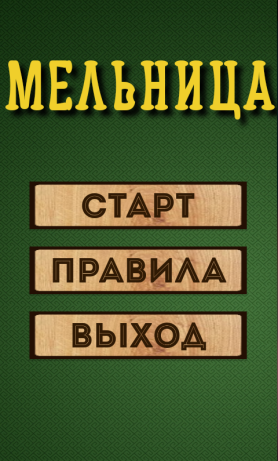
\includegraphics[scale = 0.8]{screens/MainActivity.png}
		\caption{Игровое меню} 
		\label{pic:pic_name} % название для ссылок внутри кода
	\end{center}
\end{figure}

\begin{figure}[H]
	\begin{center}
		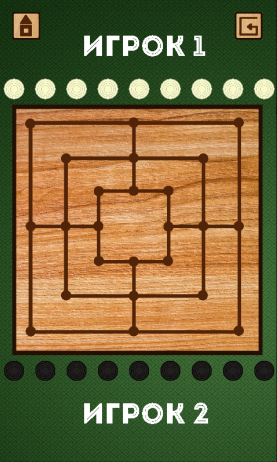
\includegraphics[scale = 0.8]{screens/GameActivity_1.png}
		\caption{Начало игры} 
		\label{pic:pic_name} % название для ссылок внутри кода
	\end{center}
\end{figure}

\begin{figure}[H]
	\begin{center}
		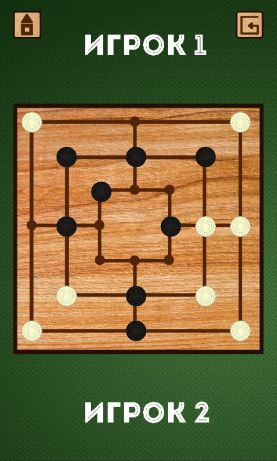
\includegraphics[scale = 0.8]{screens/GameActivity_2.png}
		\caption{Игра в процессе} 
		\label{pic:pic_name} % название для ссылок внутри кода
	\end{center}
\end{figure}

\begin{figure}[H]
	\begin{center}
		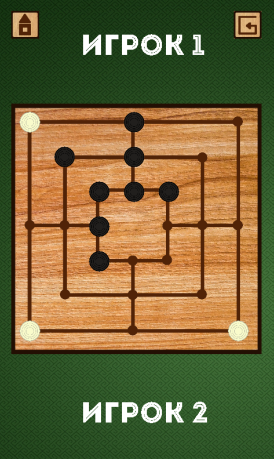
\includegraphics[scale = 0.8]{screens/GameActivity_3.png}
		\caption{Игра в процессе} 
		\label{pic:pic_name} % название для ссылок внутри кода
	\end{center}
\end{figure}

\begin{figure}[H]
	\begin{center}
		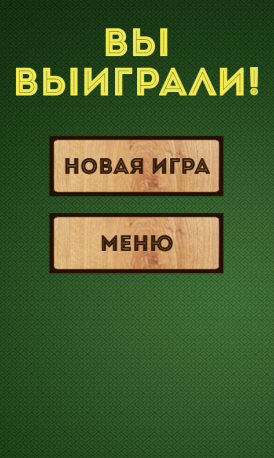
\includegraphics[scale = 0.8]{screens/EndGameActivity.png}
		\caption{Конец игры} 
		\label{pic:pic_name} % название для ссылок внутри кода
	\end{center}
\end{figure}

\begin{figure}[H]
	\begin{center}
		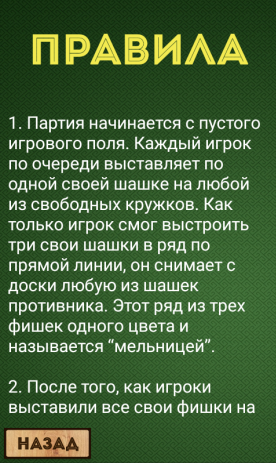
\includegraphics[scale = 0.8]{screens/RegulationsActivity.png}
		\caption{Правила} 
		\label{pic:pic_name} % название для ссылок внутри кода
	\end{center}
\end{figure}

\begin{figure}[H]
	\begin{center}
		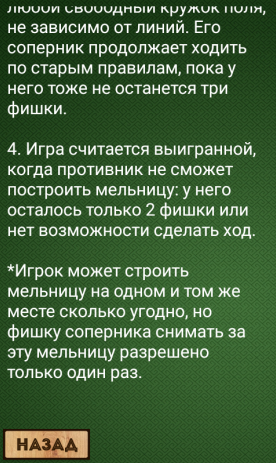
\includegraphics[scale = 0.8]{screens/RegulationsActivity_2.png}
		\caption{Правила} 
		\label{pic:pic_name} % название для ссылок внутри кода
	\end{center}
\end{figure}

\subsection{Выводы}

В данном разделе были описаны все классы, выделенные в процессе работы над проектом. Также были сделаны снимки экрана, демонстрирующие работу Android-приложения.

\section{Процесс обеспечения качества и тестирование}

\subsection{Тестирование}

Для проверки работы библиотеки использовались автоматические тесты, покрывающие основную функциональность ядра. Также в процессе разработки приложения проводилось ручное тестирование программы.

\subsection{Выводы}

В данном разделе описан процесс тестирования программы. 

\section{Выводы}

В результате работы над курсовым проектом было реализовано приложение, предназначенное для игры двух игроков в Мельницу. В процессе создания приложения был увеличен опыт написания программ на языке Java, а также получены навыки создания Android-приложения.   

\section{Приложение 1}

\captionof{lstlisting}{MillsAPI.java}
\lstinputlisting{../Core/src/main/java/ru/vlasova/mills/core/MillsAPI.java}
\parindent=1cm

\captionof{lstlisting}{Game.java}
\lstinputlisting{../Core/src/main/java/ru/vlasova/mills/core/Game.java}
\parindent=1cm

\captionof{lstlisting}{Board.java}
\lstinputlisting{../Core/src/main/java/ru/vlasova/mills/core/Board.java}
\parindent=1cm

\captionof{lstlisting}{Player.java}
\lstinputlisting{../Core/src/main/java/ru/vlasova/mills/core/Player.java}
\parindent=1cm

\captionof{lstlisting}{PlayerStatus.java}
\lstinputlisting{../Core/src/main/java/ru/vlasova/mills/core/PlayerStatus.java}
\parindent=1cm

\captionof{lstlisting}{Piece.java}
\lstinputlisting{../Core/src/main/java/ru/vlasova/mills/core/Piece.java}
\parindent=1cm

\captionof{lstlisting}{PieceStatus.java}
\lstinputlisting{../Core/src/main/java/ru/vlasova/mills/core/PieceStatus.java}
\parindent=1cm

\captionof{lstlisting}{Cell.java}
\lstinputlisting{../Core/src/main/java/ru/vlasova/mills/core/CellStatus.java}
\parindent=1cm

\captionof{lstlisting}{CellStatus.java}
\lstinputlisting{../Core/src/main/java/ru/vlasova/mills/core/CellStatus.java}
\parindent=1cm

\captionof{lstlisting}{MainActivity.java}
\lstinputlisting{../app/src/main/java/ru/vlasova/mills/android/MainActivity.java}
\parindent=1cm

\captionof{lstlisting}{GameActivity.java}
\lstinputlisting{../app/src/main/java/ru/vlasova/mills/android/GameActivity.java}
\parindent=1cm

\captionof{lstlisting}{RegulationsActivity.java}
\lstinputlisting{../app/src/main/java/ru/vlasova/mills/android/RegulationsActivity.java}
\parindent=1cm

\captionof{lstlisting}{EndGameActivity.java}
\lstinputlisting{../app/src/main/java/ru/vlasova/mills/android/EndGameActivity.java}
\parindent=1cm

\end{document}